\section{Function Definitions}
	\subsection{box function}
		1 dimension:
		\begin{equation}
			box_{1D}(u) =
			\begin{aligned}
			 & 1 && u \in [-U_b:U_b]\\
			 & 0 && otherwise
			\end{aligned}
			\label{eq:box function 1 dimension}
		\end{equation}
		N dimensions:
		\begin{equation}
		box(u) = min\left[ \sum_{k=1}^ N box_{1D}(u) \right]
		\label{eq:box function N dimensions}
		\end{equation}
	\subsection{Indicator Box function}
		\begin{equation}
			I[box]=
			\begin{aligned}
			& 0 && u \in [-U_b:U_b]\\
			& \inf && otherwise
			\end{aligned}
		\end{equation}
		
		\begin{equation}
		prox[I[box]]=
		\begin{aligned}
		& u && u \in [-U_b:U_b]\\
		& -U_b && u \in [-\inf:-U_b]\\
		& -U_b && u \in [U_b:\inf]\\
		\end{aligned}
		\end{equation}
\section{functions}

	\subsection{Conjugate of strongly convex function}
		Following lemma's are useful from 
		\begin{equation}
			f^*(x)= \underset{u \in dom(f)}{<y,x>-f(y)}
		\end{equation}
		
		If $\nabla f^*$ is lipschitz and obeys equation~\ref{eq:appendix f lip}, then $f^*$ is well defined and differentiable. (assume dom(f) is convex and closed)
		\begin{equation}
			\nabla f^*(x) = y^* = \argmax <y,x> - f(y)
		\end{equation}
		
		\begin{equation}
			|| \nabla f^*(x) - \nabla f^*(y) ||_2 \leq \mu^{-1} ||x-y||_2
			\label{eq:appendix f lip}
		\end{equation}
\clearpage
\section{Proof FBE alternate equation}

\begin{proof}
	$\varphi_{\gamma} =   f(x) + \underset{y}{\inf} \Big\{ \nabla f(x)^T(y-x) + g(y) + \frac{1}{2 \gamma} ||x-y||^2  \Big\} $
	\begin{align*}
	g^{\gamma} 	&=  \underset{y}{\inf} \big \{f(y)+\frac{1}{2 \cdot \gamma}||x-y||^2 \big \} \\
	\varphi_{\gamma} 
	&= f(x) - \frac{\gamma}{2}||\nabla f(x)||^2 + g^{\gamma} \big(x-\gamma \nabla f(x) \big) \\
	&= f(x) - \frac{\gamma}{2}||\nabla f(x)||^2 + g^{\gamma} \big(\bar{x} \big)\\
	g^{\gamma} (\bar{x})
	&=\underset{y}{\inf} \Big\{g(y)+\frac{1}{2 \gamma}||\bar{x}-y||^2 \Big\}	\\
	\frac{1}{2 \gamma}||\bar{x}-y||^2
	&=\frac{1}{2 \gamma} \Big [ (\bar{x}-y)^T(\bar{x}-y) \Big]\\
	&=\frac{1}{2 \gamma} \Big [ x^Tx - 2 x^Ty + y^Ty \Big]\\
	\bar{x}^T\bar{x}
	&=[x- \gamma \nabla f(x)]^T[x- \gamma \nabla f(x)] \\
	&= x^Tx -2x^T\nabla f(x) \gamma + \gamma^2 \nabla f(x)^T\nabla f(x)-2x^Ty \\
	&=-2(x-\gamma f\nabla(x))^Ty\\
	&=-2x^Ty + 2\gamma \nabla f(x)^Ty \\
	\frac{1}{2 \gamma}||\bar{x}-y||^2 
	& =\frac{1}{2 \gamma}[x^Tx-2x^T\nabla f(x) \gamma + \gamma^2 \nabla f(x)^T\nabla f(x) -2x^Ty + 2\gamma \nabla f(x)^Ty +y^Ty] \\
	& = \frac{1}{2 \gamma}[-2x^T\nabla f(x) \gamma  + 2\gamma \nabla f(x)^Ty + \gamma^2 \nabla f(x)^T\nabla f(x) +x^Tx -2x^Ty +y^Ty]\\
	&= \frac{1}{2 \gamma}[ 2\gamma \nabla f(x)^T(y-x) + \gamma^2||\nabla f(x)||^2 + (x-y)^T(x-y)]\\
	&= \frac{1}{2 \gamma}[ 2\gamma \nabla f(x)^T(y-x) + \gamma^2||\nabla f(x)||^2 + ||x-y||^2] \\
	&=  \nabla f(x)^T(y-x) +\frac{\gamma}{2}||\nabla f(x)||^2 + \frac{1}{2 \gamma} ||x-y||^2 \\
	g^{\gamma} (\bar{x})
	&=\underset{y}{\inf} \Big\{g(y)+ \nabla f(x)^T(y-x) +\frac{\gamma}{2}||\nabla f(x)||^2 + \frac{1}{2 \gamma} ||x-y||^2  \Big\} \\
	&= \frac{\gamma}{2}||\nabla f(x)||^2 + \underset{y}{\inf} \Big\{g(y)+ \nabla f(x)^T(y-x) + \frac{1}{2 \gamma} ||x-y||^2  \Big\} \\
	\varphi_{\gamma} 
	&= f(x) - \frac{\gamma}{2}||\nabla f(x)||^2 + g^{\gamma} \big(\bar{x} \big)\\
	&= f(x) - \frac{\gamma}{2}||\nabla f(x)||^2 +  \frac{\gamma}{2}||\nabla f(x)||^2 + \underset{y}{\inf} \Big\{g(y)+ \nabla f(x)^T(y-x) + \frac{1}{2 \gamma} ||x-y||^2  \Big\}\\
	&=   f(x) + \underset{y}{\inf} \Big\{ \nabla f(x)^T(y-x) + g(y) + \frac{1}{2 \gamma} ||x-y||^2  \Big\} 
	\end{align*}
	\label{prf:}
\end{proof}

\section{Performance measurements}
\begin{figure}[H]
	\centering
	\begin{subfigure}[b]{0.45\textwidth}
		\centering
		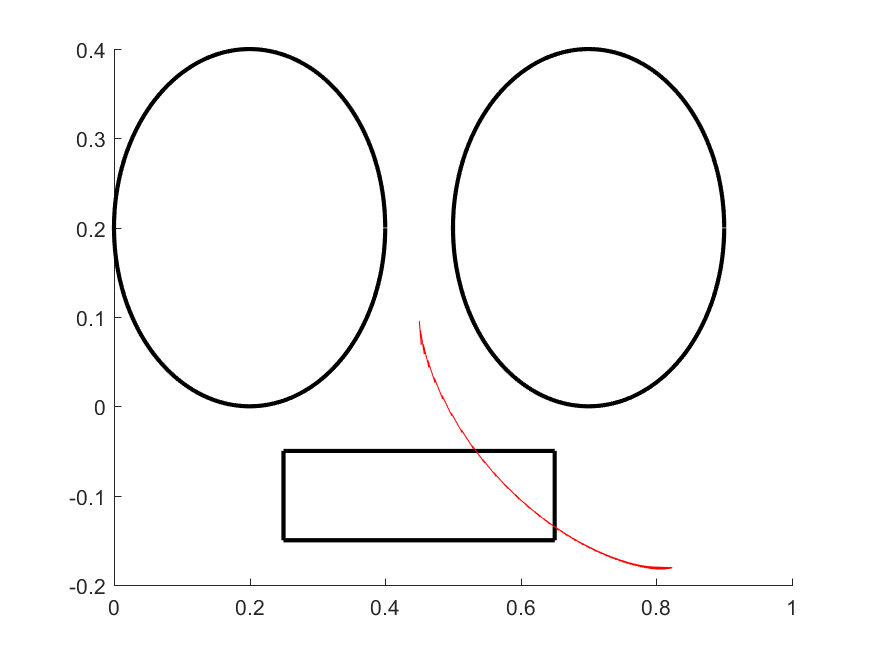
\includegraphics[width=1.2\textwidth]{demos/demo1}
		\caption{demo 1}
		\label{fig:demo 1}
	\end{subfigure}
	\hfill
	\begin{subfigure}[b]{0.45\textwidth}
		\centering
		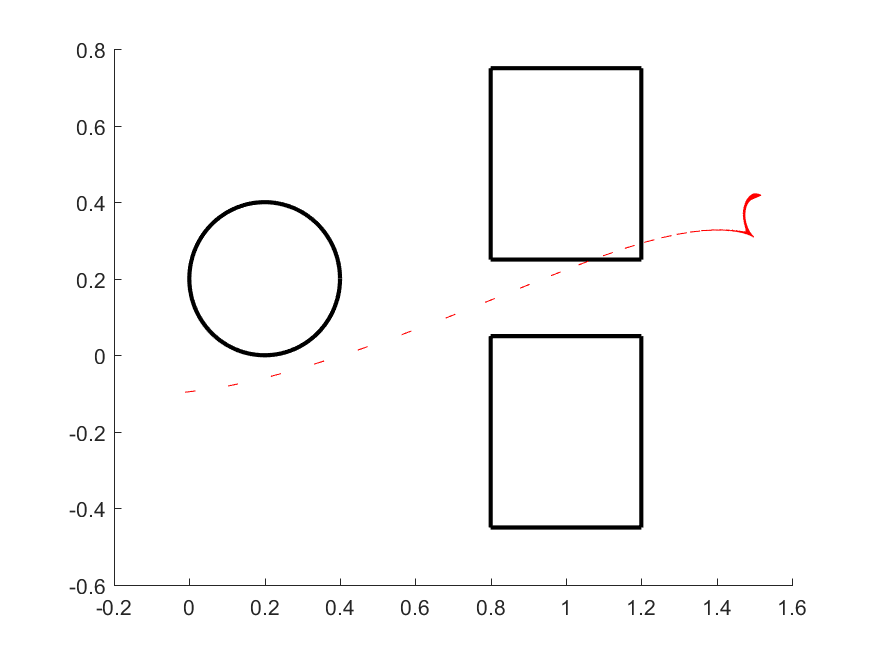
\includegraphics[width=1.2\textwidth]{demos/demo2}
		\caption{demo 2}
		\label{fig:demo 2}
	\end{subfigure}
	\begin{subfigure}[b]{0.45\textwidth}
		\centering
		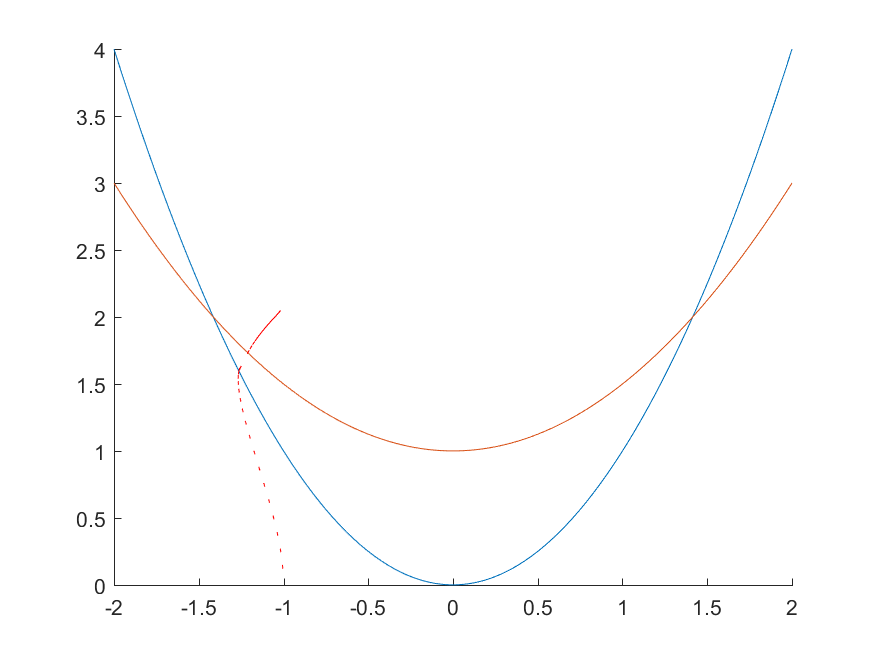
\includegraphics[width=1.2\textwidth]{demos/demo3}
		\caption{demo 3}
		\label{fig:demo 3}
	\end{subfigure}
	\hfill
	\begin{subfigure}[b]{0.45\textwidth}
		\centering
		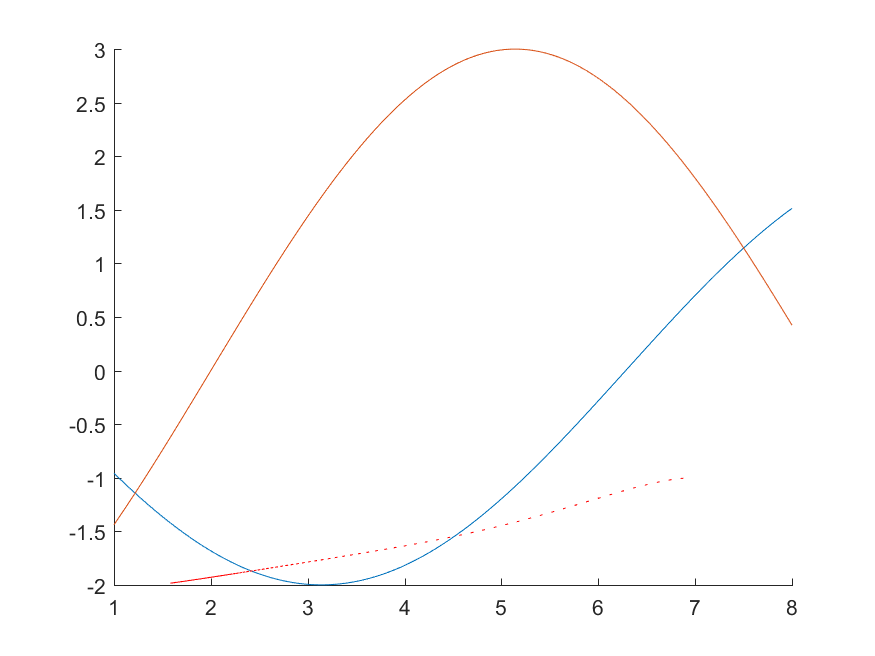
\includegraphics[width=1.2\textwidth]{demos/demo4}
		\caption{demo 4}
		\label{fig:demo 4}
	\end{subfigure}
	\begin{subfigure}[b]{0.45\textwidth}
		\centering
		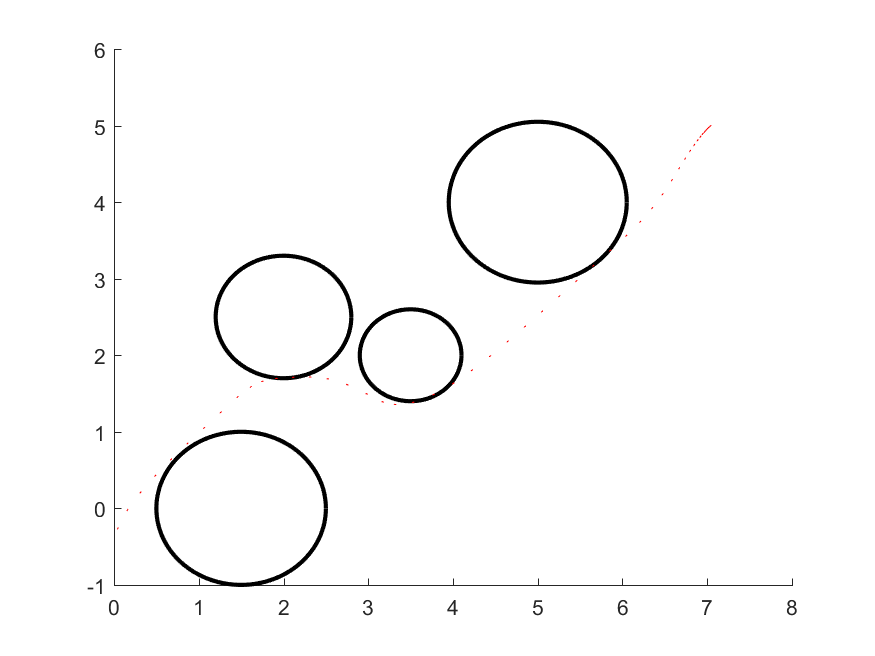
\includegraphics[width=1.2\textwidth]{demos/demo5}
		\caption{demo 5}
		\label{fig:demo 5}
	\end{subfigure}
	\caption{demos}
	\label{fig:demos}
\end{figure}

\begin{center}
	\begin{table}[H]
		\begin{tabular}{|l|c|c|c|c|}
			\hline
			&\textbf{demo5}&\textbf{demo1}&\textbf{demo2}&\textbf{demo3}\\\hline
			\textbf{nmpc-codegen}&5.37e+00&0.00e+00&4.00e-01&8.00e-01\\\hline
			\textbf{panoc Matab}&2.39e+02&1.11e+01&2.15e+01&3.74e+01\\\hline
			\textbf{fmincon:interior-point}&5.87e+02&6.27e+01&9.16e+01&1.57e+02\\\hline
			\textbf{fmincon:sqp}&1.56e+02&4.37e+01&5.83e+01&8.72e+01\\\hline
			\textbf{fmincon:active-set}&3.89e+02&5.36e+01&7.94e+01&8.81e+01\\\hline
			\textbf{OPTI:ipopt}&1.01e+03&6.54e+01&9.03e+01&2.40e+02\\\hline
		\end{tabular}
		\caption{mean time till convergence in miliseconds}
		\label{tbl:mean time till convergence}
	\end{table}
\end{center}

\begin{center}
	\begin{table}[H]
		\begin{tabular}{|l|c|c|c|c|}
			\hline
			&\textbf{demo5}&\textbf{demo2}&\textbf{demo3}\\\hline
			\textbf{nmpc-codegen}&100&100&100\\\hline
			\textbf{panoc Matab}&4610&11658&3708\\\hline
			\textbf{fmincon:interior-point}&11001&34452&10635\\\hline
			\textbf{fmincon:sqp}&2478&18401&4784\\\hline
			\textbf{fmincon:active-set}&7917&28817&5809\\\hline
			\textbf{OPTI:ipopt}&18330&29572&14618\\\hline
		\end{tabular}
		\caption{mean relative time till convergence in miliseconds}
		\label{tbl:mean relative time till convergence}
	\end{table}
\end{center}

\begin{center}
	\begin{table}[H]
		\begin{tabular}{|l|c|c|c|c|}
			\hline
			&\textbf{demo5}&\textbf{demo1}&\textbf{demo2}&\textbf{demo3}\\\hline
			\textbf{nmpc-codegen}&2.40e+01&0.00e+00&1.40e+01&1.40e+01\\\hline
			\textbf{panoc Matab}&2.51e+03&7.08e+01&3.44e+02&8.28e+02\\\hline
			\textbf{fmincon:interior-point}&1.13e+04&2.71e+02&3.88e+02&6.22e+02\\\hline
			\textbf{fmincon:sqp}&3.90e+02&9.18e+01&2.36e+02&5.89e+02\\\hline
			\textbf{fmincon:active-set}&2.85e+03&1.22e+02&7.39e+02&6.44e+02\\\hline
			\textbf{OPTI:ipopt}&3.17e+03&2.30e+02&8.24e+02&1.36e+03\\\hline
		\end{tabular}
		\caption{max time till convergence in miliseconds}
		\label{tbl:max time till convergence}
	\end{table}
\end{center}

\begin{center}
	\begin{table}[H]
		\begin{tabular}{|l|	c|c|c|c|}
			\hline
			&\textbf{demo5}&\textbf{demo1}&\textbf{demo2}&\textbf{demo3}\\\hline
			\textbf{nmpc-codegen}&0.00e+00&0.00e+00&0.00e+00&0.00e+00\\\hline
			\textbf{panoc Matab}&1.44e+01&7.86e+00&7.64e+00&1.18e+01\\\hline
			\textbf{fmincon:interior-point}&1.02e+02&3.87e+01&3.82e+01&3.66e+01\\\hline
			\textbf{fmincon:sqp}&5.13e+01&3.40e+01&3.41e+01&3.78e+01\\\hline
			\textbf{fmincon:active-set}&7.60e+01&4.31e+01&4.50e+01&5.35e+01\\\hline
			\textbf{OPTI:ipopt}&1.23e+02&5.01e+01&5.05e+01&5.86e+01\\\hline
		\end{tabular}
		\caption{min time till convergence in miliseconds}
		\label{tbl:min time till convergence}
	\end{table}
\end{center}